%==============================


%fig 11.1 pg 406
\begin{figure}
\centering
\begin{tikzpicture}[]
\draw[-stealth] (0,0) -- (5,0) node[below]{$z$};
\draw[dashed] (0,0.5) -- (5,0.5);
\draw[thick,->-=0.5] (0,0.5) to [out=0,in=-120] (5,4);
\draw[dashed] (3.25,0.5) -- (5,4);
\draw[]([shift={(0:0.5)}]3.25,0.5) arc (0:60:0.5) node[pos=0.5,right]{$\theta$};
\draw[stealth-stealth] (0.4,0) -- (0.4,0.5) node[pos=0.5,left]{$b$};
\draw[] (3.5,0) node[circle,inner sep= 1.5pt,fill=black]{} node[below]{\RL{نقطہ بکھراو}};
\end{tikzpicture}
\caption{
کلاسیکی مسئلہ بکھراو، جس میں ٹکراو مقدار معلوم \عددی{b} اور زاویہ بکھراو \عددی{\theta} کی وضاحت کی گئی ہے۔
}
\label{
شکل_بکھراو_کلاسیکی_ٹکراو_اور_زاویہ
}
\end{figure}


%==============================


%fig 11.2 pg 407
\begin{figure}
\centering
\pgfmathsetmacro{\r}{1.5}
\pgfmathsetmacro{\ang}{35}
\pgfmathsetmacro{\b}{\r*sin(\ang)}
\pgfmathsetmacro{\c}{\r*cos(\ang)}
\begin{tikzpicture}[]
\draw[] (0,0) node[circle, inner sep=1.5pt, fill=black]{} circle (\r);
\draw[-stealth] (-5,0) -- (2,0) node[below]{$z$};
\draw[stealth-stealth] (-4.4,0) --++ (0,\b) node[pos=0.5,left]{$b$};
\draw[thick,-stealth] (-5,\b) -- (-\c,\b) --++ (180-2*\ang:2);
\draw[dashed] (-\c, \b) --++ (1.25,0);
\draw[dashed] (0,0) --++ (180-\ang:3) node[pos=0.25,shift={(90-\ang:0.75em)}]{$R$};
\draw[] ([shift={(180-\ang:0.5)}]0,0) arc (180-\ang:180:0.5) node[pos=0.4,left]{$\alpha$};
\draw[] ([shift={(180-\ang:0.5)}]-\c,\b) arc (180-\ang:180:0.5) node[pos=0.4,left]{$\alpha$};
\draw[] ([shift={(180-2*\ang:0.4)}]-\c,\b) arc (180-2*\ang:180-\ang:0.4) node[pos=0.5,shift={(180-1.5*\ang:0.75em)}]{$\alpha$};
\draw[] ([shift={(0:0.75)}]-\c,\b) arc (0:180-2*\ang:0.75) node[pos=0.5,above]{$\theta$};
\end{tikzpicture}
\caption{	
سخت کرہ سے لچکدار بکھراو۔
}
\label{
شکل_بکھراو_سخت_کرہ_لچکدار
}
\end{figure}



%==============================


%fig 11.3 pg 408
\begin{figure}
\centering
\pgfmathsetmacro{\r}{2}
\pgfmathsetmacro{\ta}{30}
\pgfmathsetmacro{\tb}{40}
\pgfmathsetmacro{\pa}{40}
\pgfmathsetmacro{\pb}{80}
\pgfmathsetmacro{\ia}{0.5}
\pgfmathsetmacro{\ib}{0.3}
\pgfmathsetmacro{\tcc}{\ta+(\tb-\ta)/2}
\pgfmathsetmacro{\tdd}{\pa+(\pb-\pa)/2}
\begin{tikzpicture}[declare function={fa(\t,\p)=\r*sin(\t)*cos(\p);fb(\t,\p)=\r*sin(\t)*sin(\p);fc(\t,\p)=\r*cos(\t);}, 
x={(0cm,-0.25cm)}, y={(1cm,0cm)}, z={(0cm,1cm)}]
\begin{scope}[rotate=-90]
\draw[] plot [domain=0:360,smooth]({fa(\x,90)},{fb(\x,90)},{fc(\x,90)});
\draw[] plot [domain=-90:90,smooth]({fa(\ta,\x)},{fb(\ta,\x)},{fc(\ta,\x)});
\draw[] plot [domain=-90:90,smooth]({fa(\tb,\x)},{fb(\tb,\x)},{fc(\tb,\x)});
%\draw[dashed] plot [domain=90:270]({fa(\ta,\x)},{fb(\ta,\x)},{fc(\ta,\x)});
%\draw[dashed] plot [domain=90:270]({fa(\tb,\x)},{fb(\tb,\x)},{fc(\tb,\x)});
\draw[] plot [domain=\ta:\tb]({fa(\x,\pa)},{fb(\x,\pa)},{fc(\x,\pa)});
\draw[] plot [domain=\ta:\tb]({fa(\x,\pb)},{fb(\x,\pb)},{fc(\x,\pb)});
\coordinate (tta) at ({fa(\ta,\pa)},{fb(\ta,\pa)},{fc(\ta,\pa)});
\coordinate (ttb) at ({fa(\ta,\pb)},{fb(\ta,\pb)},{fc(\ta,\pb)});
\coordinate (ppa) at ({fa(\tb,\pa)},{fb(\tb,\pa)},{fc(\tb,\pa)});
\coordinate (ppb) at ({fa(\tb,\pb)},{fb(\tb,\pb)},{fc(\tb,\pb)});
\draw[] (tta) -- (0,0,0);
\draw[] (ttb) -- (0,0,0);
\draw[] (ppa) -- (0,0,0);
\draw[] (ppb) -- (0,0,0);
\draw[] (0,0,0) node[circle,inner sep=1.5pt,fill=black]{} -- ({fa(\ta,-90)},{fb(\ta,-90)},{fc(\ta,-90)});
\draw[] (0,0,0) -- ({fa(\tb,-90)},{fb(\tb,-90)},{fc(\tb,-90)});
\draw[] (0,0,-6) -- (0,0,2.5);
\draw[] plot [domain=0:\ta] ({0.4*fa(\x,-90)},{0.4*fb(\x,-90)},{0.4*fc(\x,-90)});
\draw[] ({0.4*fa(\ta/2,-90)},{0.4*fb(\ta/2,-90)},{0.4*fc(\ta/2,-90)}) node[right,yshift=0.25em]{$\theta$};
\draw[] plot [domain=\ta:\tb]({0.5*fa(\x,-90)},{0.5*fb(\x,-90)},{0.5*fc(\x,-90)});
\draw[] ({0.5*fa(\ta,-90)},{0.5*fb(\ta,-90)},{0.5*fc(\ta,-90)}) node[pin={[]160:{$\dif\theta$}}]{};
\draw[] plot [domain=0:360] ({\ia*fa(90,\x)},{\ia*fb(90,\x)},{-5+\ia*fc(90,\x)});
\draw[] plot [domain=0:360] ({\ib*fa(90,\x)},{\ib*fb(90,\x)},{-5+\ib*fc(90,\x)});
\coordinate (iia) at ({\ia*fa(90,\pa)},{\ia*fb(90,\pa)},{-5+\ia*fc(90,\pa)});
\coordinate (iib) at ({\ib*fa(90,\pa)},{\ib*fb(90,\pa)},{-5+\ib*fc(90,\pa)});
\coordinate (iic) at ({\ia*fa(90,\pb)},{\ia*fb(90,\pb)},{-5+\ia*fc(90,\pb)});
\coordinate (iid) at ({\ib*fa(90,\pb)},{\ib*fb(90,\pb)},{-5+\ib*fc(90,\pb)});
\draw[] (iia) -- (iib);
\draw[] (iic) -- (iid);
\path[name path=za] plot [domain=\pa:\pb] ({\ia*fa(90,\x)},{\ia*fb(90,\x)},{-5+\ia*fc(90,\x)});
\path[name path=zb] plot [domain=\pa:\pb] ({\ib*fa(90,\x)},{\ib*fb(90,\x)},{-5+\ib*fc(90,\x)});
\tikzfillbetween[of=za and zb]{black};
\path[name path=zc] plot [domain=\pa:\pb,smooth]({fa(\ta,\x)},{fb(\ta,\x)},{fc(\ta,\x)});
\path[name path=zd] plot [domain=\pa:\pb,smooth]({fa(\tb,\x)},{fb(\tb,\x)},{fc(\tb,\x)});
\tikzfillbetween[of=zc and zd]{black};
\draw[thick] ($(iia)!0.5!(iid)$) coordinate(bba) --++ (0,0,-1) coordinate(bbb);
\draw[thick] ($(iia)!0.5!(iid)$) --++ (0,0,4.5) coordinate(kleft);
\draw[line width=2pt,-stealth,white] ($(tta)!0.5!(ppb)$) coordinate(kright) --({1.75*fa(\tcc,\tdd)},{1.75*fb(\tcc,\tdd)},{1.75*fc(\tcc,\tdd)});
\draw[thick,-stealth] ($(tta)!0.5!(ppb)$) coordinate(kright) --({1.75*fa(\tcc,\tdd)},{1.75*fb(\tcc,\tdd)},{1.75*fc(\tcc,\tdd)});
\draw[thick] (kleft) to [out=90,in=245] (kright);
\draw[stealth-,shorten <=1.5pt] ($(iia)!0.5!(iic)$) --++ (0.5,0.5) node[below]{$\dif\sigma$};
\draw[stealth-stealth] (0,0,-5.75) -- ($(bba)!(0,0,-5.75)!(bbb)$) node[pos=0.5,left]{$b$};
\draw[] (iib) -- (0,0,-5);
\draw[] (iid) -- (0,0,-5);
\path[]($(iia)!0.5!(iid)$)--(0,0,-5)coordinate[pos=0.5](kkphi);
\draw[] (kkphi) to [out=90,in=-90] ++ (0,-1,1)node[right]{$\dif \phi$};
\draw[] plot [domain=\ta-15:\tb+7] ({0.3*fa(\x,90)},{0.3*fb(\x,90)},{0.3*fc(\x,90)});
\draw[] plot [domain=\ta-15:\tb+7] ({0.35*fa(\x,90)},{0.35*fb(\x,90)},{0.35*fc(\x,90)});
\draw[]({0.35*fa(\tcc,90)},{0.35*fb(\tcc,90)},{0.35*fc(\tcc,90)})--++(0,0.75,0.3)node[below]{$\dif\Omega$};
\end{scope}
\end{tikzpicture}
\caption{
رقبہ \عددی{\dif \sigma} میں آمدی ذرات ٹھوس زاویہ \عددی{\dif\Omega} میں بکھرتے ہیں۔
}
\label{
شکل_بکھراو_آمدی_اور_ٹھوس_زاویہ
}
\end{figure}




%==============================


%fig 11.4 pg 410
\begin{figure}
\centering
\pgfmathsetmacro{\r}{0.5}
\pgfmathsetmacro{\anga}{35}
\pgfmathsetmacro{\angb}{110}
\pgfmathsetmacro{\angc}{10}
\pgfmathsetmacro{\a}{\r/3}
\begin{tikzpicture}
\draw[-stealth] (-6,0) -- (2.75,0) node[below]{$z$};
\foreach \n in {1,2,3,4}{\draw (0,0) circle (\n*\r);}
\draw[fill=black] (0,0) circle (1.5pt);
\draw[] (0,0) circle (3.5pt);
\draw[] (0,0) --++ (\anga:2.5);
\draw[] (0,0) ++ (\angb:1.5*\r) ++ (\angb-90:\a) --++ (\angb-\angc:3*\r) --++ (\angb-90:\r/2) coordinate(za);
\draw[] (0,0) ++ (\angb:1.5*\r) ++ (\angb+90:\a) --++ (\angb+\angc:3*\r) --++ (\angb+90:\r/2) coordinate(zb);
\draw[] (\angb:5.5*\r) -- (za) node[right]{$e^{ikr}$};
\draw[] (\angb:5.5*\r) -- (zb);
\draw[] (\anga/2:1.5*\r) node[]{$\theta$};
\foreach \n in {1,2,3,4,5} {\draw[] (-3-\n*\r,1.5) --++ (0,-3);}
\draw[] (-3-2.5*\r,-\r) --++ (2.5*\r,0) --++ (0,0.25*\r) coordinate(zc);
\draw[] (-3-2.5*\r,-1.5*\r) --++ (2.5*\r,0) --++ (0,-0.25*\r) coordinate(zd);
\draw[] (-3-2.5*\r,-1.25*\r) ++ (3*\r,0) coordinate(ze);
\draw[] (zc) -- (ze);
\draw[] (zd) -- (ze); 
\draw[] (-3-3*\r,-1.5) node[below]{$e^{ikz}$};
\end{tikzpicture}
\caption{	
امواج کا بکھراو؛ آمدی مستوی موج    رخصتی کروی موج پیدا کرتی ہے۔
}
\label{
شکل_بکھراو_مستوی_آمدی_کروی_رخصتی
}
\end{figure}




%==============================


%fig 11.5 pg 411
\begin{figure}
\centering
\pgfmathsetmacro{\ra}{1.5}
\pgfmathsetmacro{\rb}{1}
\pgfmathsetmacro{\anga}{70}
\pgfmathsetmacro{\angb}{-30}
\pgfmathsetmacro{\d}{3}
\pgfmathsetmacro{\angc}{(\anga+\angb)/2}
\pgfmathsetmacro{\rc}{(\ra+\rb)/2}
\begin{tikzpicture}
\draw[fill=lgray,opacity=0.5] ([shift={(\angb:\ra)}]0,0) arc (\angb:\anga:\ra) coordinate(za)coordinate[pos=0](zaa)--(\anga:\rb) 
([shift={(\anga:\rb)}]0,0) arc (\anga:\angb:\rb) coordinate(zbb)coordinate[pos=0](zb)--(\angb:\ra);

\draw[] ([shift={(\angb:\ra)}]\d,0) arc (\angb:\anga:\ra) coordinate(zc)coordinate[pos=0](zcc);
\draw[dashed] ([shift={(\angb:\rb)}]\d,0) arc (\angb:\anga:\rb) coordinate(zd)coordinate[pos=0](zdd);
\draw[dashed] (zc) -- (zd);
\draw[dashed] (zcc) -- (zdd);
\draw(za)--(zc);
\draw(zaa)--(zcc);
\draw[dashed](zb)--(zd);
\draw[dashed](zbb)--(zdd);
\draw[decorate,decoration={brace,amplitude=5pt,raise=4pt,mirror}] (zaa)--(zcc) node[pos=0.5,yshift=-1.5em]{$v\dif t$};
\draw[] (\angc:\rc) node[pin={-135:{$\dif \sigma$}}]{};
\draw[-stealth] (\angc:\rc) ++ (\d+0.5,0) --++ (1.5,0) node[pos=0.5,above]{$v$};
\end{tikzpicture}
\caption{	
وقت \عددی{\dif t} کے دوران رقبہ \عددی{\dif\sigma} سے گزرتی  ہوئی آمدی  شعاع کا حجم \عددی{\dif V} ہے۔
}
\label{
شکل_بکھراو_رقبہ_حجم_شعاع
}
\end{figure}



%==============================


%fig 11.6 pg 412
\begin{figure}
\centering
\begin{tikzpicture}
\draw[] (0,0) node[]{$V=0$} circle (0.6);
\draw[] (0,0) node[]{$V=0$} circle (2);
\draw[stealth-] (-160:0.6) to [out=-160,in=0] ++ (-1.5,-0.75) node[left]{\RL{خطہ بکھراو}};
\draw[] (0,1) node[yshift=-0.25em]{$V\equiv 0$} node[above]{\RL{درمیانہ خطہ}};
\draw[] (3,0.5) node[]{\RL{اشعاعی خطہ}} node[below,yshift=-0.25em]{$(kr\gg 1)$};
\end{tikzpicture}
\caption{	
مقمای مخفیہ سے بکھراو؛ خطہ بکھراو، درمیانہ خطہ، اور اشعاعی خطہ۔
}
\label{
شکل_بکھراو_تین_خطے
}
\end{figure}



%==============================


%fig 11.7 pg 417
\begin{figure}
\centering
\pgfmathsetmacro{\a}{0.8}
\pgfmathsetmacro{\b}{100}
\begin{tikzpicture}[declare function={f(\x)=1.5*e^(\a*\x)*cos(\b*\x);}]
\fill[lgray] (0,0) rectangle (0.25,2.75);
\draw[-stealth] (-4.5,0) -- (1,0) node[below]{$x$};
\draw[] (0,-0.75) -- (0,3);
\draw[very thick,stealth-stealth] plot [domain=-6:0]({\x},{f(\x)})-- (0,3) node[left]{$V$};
\draw(-3.75,0)--++(0,-0.1)node[below]{$a$};
\draw[stealth-](-3.5,2.5)--++(1,0)node[right]{$Be^{-ikx}$};
\draw[-stealth](-3.5,1.5)--++(1,0)node[right]{$Ae^{ikx}$};
\end{tikzpicture}
\caption{	
مقامی مخفیہ، جس کے  دائیں جانب ایک   لامتناہی دیوار  پائی جاتی ہے، سے یک بعدی بکھراو۔
}
\label{
شکل_بکھراو_یک_بعدی_مقامی_مخفیہ
}
\end{figure}

%=======================================


%fig 11.8 pg 422
\begin{figure}
\centering
\pgfmathsetmacro{\r}{0.6}
\pgfmathsetmacro{\ra}{0.85}
\pgfmathsetmacro{\anga}{-117}
\pgfmathsetmacro{\angb}{-57}
\begin{tikzpicture}
\draw[-stealth] (0,0) -- (-1.5,-1);
\draw[-stealth] (0,0) -- (3,0);
\draw[-stealth] (0,0) -- (0,3);
\draw[thick,-stealth] (0,0) -- (0,2.5) node[pos=0.5,left]{$\kvec{r}$};
\draw[thick,-stealth] (0,0) -- (2,2) node[above]{$\kvec{s}$};
\draw[dashed] (2,2) -- (2,-1) -- (0,0);
\RightAngle {(2,2)}{ (2,-1)}{ (0,0)}
\draw[] ([shift={(48:\r)}]0,0) arc (48:90:\r) node[pos=0.5,shift={(70:0.75em)}]{$\theta$};
\draw[] ([shift={(\anga:\ra)}]0,0.5) arc (\anga:\angb:\ra) node[pos=0.5,shift={(-90:0.75em)}]{$\phi$};
\end{tikzpicture}
\caption{	
موزوں محدد برائے مساوات \حوالہء{11.58} کا تکمل۔
}
\label{
شکل_بکھراو_موزوں_محدد
}
\end{figure}



%=======================================


%fig 11.9 pg 423
\begin{figure}
\centering
\pgfmathsetmacro{\r}{0.2}
\begin{tikzpicture}
\draw[-stealth] (-3,0) -- (3.5,0) node[below]{\RL{حقیقی \عددی{(s)}}};
\draw[-stealth] (0,-0.25) -- (0,1.5) node[left]{\RL{خیالی \عددی{(s)}}};
\draw[](-2,0)node[circle,fill=black,inner sep=1.5pt]{}node[below,yshift=-0.5em]{$s=-k$};
\draw[](2,0)node[circle,fill=black,inner sep=1.5pt]{}node[below,yshift=-0.5em]{$s=+k$};
\draw[very thick,-stealth] (-2.75,0) -- (-2-\r,0) ([shift={(180:\r)}]-2,0) arc (180:0:\r) -- (2-\r,0)  ([shift={(180:\r)}]2,0) arc (180:360:\r) -- (3,0);
\end{tikzpicture}
\caption{	
ارتفاعی تکمل (مساوات \حوالہء{11.61}) میں ہمیں  قطبین کے  اطراف سے گزرنا ہو گا ۔
}
\label{
شکل_بکھراو_قطبین-اطراف_گزرنا
}
\end{figure}



%=======================================


%fig 11.10 pg 423
\begin{figure}
\centering
\begin{subfigure}{0.45\textwidth}
\centering
\pgfmathsetmacro{\r}{0.2}
\pgfmathsetmacro{\p}{0.75}
\begin{tikzpicture}
\draw[] (-1.5,0) -- (1.5,0);
\draw[](-\p,0)node[circle,fill=black,inner sep=1.5pt]{};
\draw[](\p,0)node[circle,fill=black,inner sep=1.5pt]{};
\draw[very thick,->-=0.55] (-1.25,0) -- (-\p-\r,0) ([shift={(180:\r)}]-\p,0) arc (180:0:\r) -- (\p-\r,0)  ([shift={(180:\r)}]\p,0) arc (180:360:\r) -- (1.25,0);
\draw[very thick,->-=0.5] ([shift={(0:1.25)}]0,0) arc (0:180:1.25); 
\end{tikzpicture}
\caption{}
\end{subfigure}\hfill
\begin{subfigure}{0.45\textwidth}
\centering
\pgfmathsetmacro{\r}{0.2}
\pgfmathsetmacro{\p}{0.75}
\begin{tikzpicture}
\draw[] (-1.5,0) -- (1.5,0);
\draw[](-\p,0)node[circle,fill=black,inner sep=1.5pt]{};
\draw[](\p,0)node[circle,fill=black,inner sep=1.5pt]{};
\draw[very thick,->-=0.55] (-1.25,0) -- (-\p-\r,0) ([shift={(180:\r)}]-\p,0) arc (180:0:\r) -- (\p-\r,0)  ([shift={(180:\r)}]\p,0) arc (180:360:\r) -- (1.25,0);
\draw[very thick,-<-=0.5] ([shift={(180:1.25)}]0,0) arc (180:360:1.25); 
\end{tikzpicture}
\caption{}
\end{subfigure}
\caption{	
مساوات \حوالہء{11.63} اور مساوات \حوالہء{11.64} کے   خط  ارتفاع  کو بند کرنا دکھایا گیا ہے۔
}
\label{
شکل_بکھراو_ارتفاعی_تکملات_بند
}
\end{figure}

%=======================================


%fig 11.11 pg 426
\begin{figure}
\centering
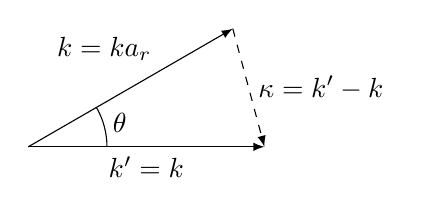
\begin{tikzpicture}
\draw[-latex] (0,0) -- (3,0) node[pos=0.5,below]{$\kvec{k}'=k\az$}coordinate(aa);
\draw[-latex] (0,0) --++ (30:3) node[pos=0.65,above left]{$\kvec{k}=k\kvec{a}_r$}coordinate(bb);
\draw[-latex,dashed] (bb)--(aa)node[pos=0.5,right]{$\kvec{\kappa}=\kvec{k}'-\kvec{k}$};
\draw([shift={(0:1)}]0,0) arc (0:30:1)node[pos=0.6,right]{$\theta$};
\end{tikzpicture}
\caption{	
بارن تخمین میں دو تفاعل موج: \عددی{k'} آمدی رخ جبکہ \عددی{k} بکھراو رخ ہے۔
}
\label{
شکل_بکھراو_آمدی_بکھراو_رخ
}
\end{figure}



%=======================================


%fig 11.12 pg 429
\begin{figure}
\centering
\begin{tikzpicture}
\pgfmathsetmacro{\ang}{atan(1/2.5)}
\draw[] (0,0) -- (6,0) node[pos=0.55, circle, inner sep=1.5pt,fill=black]{} node[pos=0.55, below]{\RL{نقطہ بکھراو}} ;
\draw[dashed] (0,1) -- (6,1) node[pos=0.5, circle, inner sep=1.5pt,fill=black]{};
\draw[thick,-stealth] (0,1) to [out=0,in=-160] (6,2) node[above]{\RL{اصل خط حرکت}};
\draw[-stealth] (3,1) -- (3,2) node[above]{$F_{\perp}$}; 
\draw[dashed] (3.5,1) -- (6,2);
\draw[] ([shift={(0:1)}]3.5,1) arc (0:\ang:1) node[pos=0.6,right]{$\theta$};
\draw[stealth-stealth] (0.25,0) --++ (0,1) node[pos=0.5,left]{$b$};
\end{tikzpicture}
\caption{	
 ذرہ  کو منتقل معیار حرکت کا حساب کرتے ہوئے،تخمین ضرب کی ترکیب  میں فرض کیا  جاتا ہے کہ ذرہ بغیر  مڑے سیدھی لکیر پر حرکت کیے جاتا ہے۔
}
\label{
شکل_بکھراو_تخمین_ضرب
}
\end{figure}




%=======================================


%fig 11.13 pg 430
\begin{figure}
\centering
\begin{tikzpicture}
\pgfmathsetmacro{\a}{1.25}
\pgfmathsetmacro{\r}{0.75}
\pgfmathsetmacro{\d}{0.25}
\draw[->-=0.6] (0,0) node[left]{$\psi=$} --++ (\a,0) node[pos=0.5,below]{$\psi_0$};
\draw[] (\a +\d,0) node[]{$+$};
\draw[->-=0.25] (\a+2*\d,0) --++ (\a,0) node[pos=0.25,below]{$\psi_0$} coordinate(aa);
\draw[] (aa) node[circle, inner sep= 1.5pt, fill=black]{} node[below]{$V$} circle (\r);
\draw[] (aa) --++ (30:1.25) node[pos=0.25,shift={(-60:0.5em)}]{$g$};
\draw[] (2*\a +4*\d+\r,0) node[]{$+$};
\draw[->-=0.3] (2*\a +5*\d+\r,0) --++ (\a,0) node[pos=0.3,below,xshift=-0.1em]{$\psi_0$} coordinate(aa);
\draw[] (aa) node[circle, inner sep= 1.5pt, fill=black]{} node[below]{$V$} circle (\r);
\draw[] (aa) --++ (20:0.5) node[pos=0.5,shift={(110:0.5em)}]{$g$} node[circle, inner sep=1.5pt,fill=black]{} node[below]{$V$} --++ (80:1) node[pos=0.5,right]{$g$};
\draw[] (3*\a +6*\d+2*\r,0) node[]{$+$};
\draw[->-=0.3] (3*\a +7*\d+2*\r,0) --++ (0.75*\a,0) node[pos=0.3,below,xshift=-0.1em]{$\psi_0$} node[circle, inner sep= 1.5pt, fill=black]{} node[above]{$V$}coordinate(bb); 
\draw[] (4*\a +7*\d+2*\r,0) coordinate(aa) circle (\r);
\draw[] (bb) --++ (-40:0.5) node[pos=0.5,shift={(-130:0.5em)}]{$g$} node[circle, inner sep=1.5pt,fill=black]{} node[below]{$V$} --++ (45:0.75) node[pos=0.5,shift={(-45:0.5em)}]{$g$}node[circle, inner sep=1.5pt,fill=black]{}node[above left]{$V$}--++(-10:1)node[pos=0.75,above]{$g$};
\draw[] (5*\a +7*\d+3*\r,0) node[]{$+\cdots$};
\end{tikzpicture}
\caption{	
بارن تسلسل (مساوات \حوالہء{11.101}) کا  نظیری مفہوم۔
}
\label{
شکل_بکھراو_نظیری_مفہوم
}
\end{figure}



%=======================================


%fig 12.1 pg 433
\begin{figure}
\centering
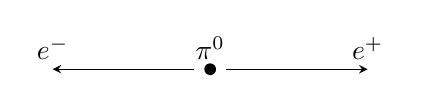
\begin{tikzpicture}
\draw[-stealth] (-0.2,0) -- (-2,0) node[above]{$e^{-}$};
\draw[-stealth] (0.2,0) -- (2,0) node[above]{$e^{+}$};
\draw[] (0,0) node[circle, inner sep=1.5pt, fill=black]{} node[above]{$\pi^{0}$};
\end{tikzpicture}
\caption{	
آئنشٹائن، پوڈلسکی و  روزن  تضاد کا بوہم انداز۔ساکن \عددی{\pi^0}  کا تنزل الیکٹران و  ضد الیکٹران  جوڑی میں ہوتا ہے۔
}
\label{
شکل_بکھراو_بوہم_تنزل
}
\end{figure}




%=======================================


%fig 12.2 pg 436
\begin{figure}
\centering
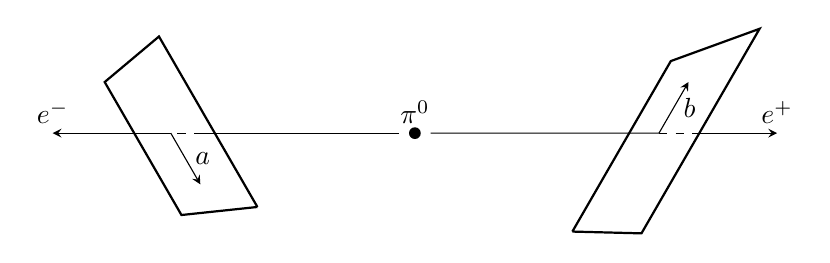
\begin{tikzpicture}
\pgfmathsetmacro{\anga}{60}
\pgfmathsetmacro{\angb}{180-\anga}
\pgfmathsetmacro{\a}{2}
\pgfmathsetmacro{\b}{1.25}
\pgfmathsetmacro{\c}{1.2}
\pgfmathsetmacro{\d}{3}
\draw[-stealth] (0.2,0) -- (3.1,0) --++ (\anga:0.75) node[pos=0.5,right]{$\kvec{b}$};
\draw[dashed](3.1,0)--++(0.5,0);
\draw[-stealth] (3.6,0) -- (4.6,0) node[above]{$e^{+}$};
\draw[] (-0.2,0) -- (-2.7,0);
\draw[dashed] (-2.7,0) -- (-3.1,0) coordinate(kl);
\draw[-stealth] (kl) --++ (\angb:-0.75) node[pos=0.5, right]{$\kvec{a}$};
\draw[-stealth] (kl) --++ (-1.5,0) node[above]{$e^{-}$};
\draw[] (0,0) node[circle, inner sep=1.5pt, fill=black]{} node[above]{$\pi^{0}$};
\draw[thick] (\a,-\b) coordinate(s) --++ (\anga:2*\b) --++ (20:\c) --++ (\anga:-\d) -- (s);
\draw[thick] (-\a,-0.75*\b) coordinate(ss) --++ (\angb:2*\b) --++ (-140:0.75*\c) --++ (\angb:-0.65*\d) -- (ss);
\end{tikzpicture}
\caption{	
آئنشٹائن، پوڈلسکی و  روزن  تضاد کا بل  انداز۔کاشف آزادانہ طور پر \عددی{\kvec{a}} اور \عددی{\kvec{b}} رخ سمت بند ہیں۔
}
\label{
شکل_بکھراو_بل_انداز
}
\end{figure}



%=======================================


%fig 12.3 pg 438
\begin{figure}
\centering
\begin{tikzpicture}
\draw[-stealth] (0,0) -- (3,0) node[below]{$\kvec{a}$};
\draw[-stealth] (0,0) -- (0,3) node[left]{$\kvec{b}$};
\draw[-stealth] (0,0) --++ (45:2.5) node[above]{$\kvec{c}$};
\draw[] ([shift={(0:0.5)}]0,0) arc (0:45:0.5) node[pos=0.6,right]{$45^{o}$};
\draw[] ([shift={(45:0.75)}]0,0) arc (45:90:0.75) node[pos=0.5,shift={(67.5:0.3)}]{$45^{o}$};
\end{tikzpicture}
\caption{	
کاشف کو یوں سمت بند کیا گیا ہے کہ بل عدم مساوات کی کوانٹائی   خلاف ورزی   ظاہر ہو۔
}
\label{
شکل_بکھراو_بل_عدم-مساوات
}
\end{figure}

%=======================================


%fig 12.4 pg 439
\begin{figure}
\centering
\pgfmathsetmacro{\ra}{0.3}
\pgfmathsetmacro{\rb}{0.5}
\begin{tikzpicture}[declare function={fa(\t)=\ra*cos(\t); fb(\t)=\rb*sin(\t);}]
%\draw[] (0,0) circle (0.3cm and 0.5cm);
\draw[] plot[domain=120:420]({fa(\x)},{fb(\x)});
\draw[thick] ({fa(120)},{fb(120)})coordinate(bba) -- ({fa(420)},{fb(420)})coordinate(bbb)coordinate[pos=0.5](bbc);
\draw[thick](bba) to [out=90, in=90] (bbb);
\draw(bbc) to [out=90,in=45]++(0.3,0.3);
\draw(bbc) to [out=90,in=135]++(-0.3,0.3);
\draw[thin](bbc)--({fa(270)},{fb(270)});
\draw[] ({fa(35)},{fb(35)}) to [out=70,in=-160] ++ (0.2,0.2);
\draw[] ({fa(145)},{fb(145)}) to [out=110,in=-20] ++ (-0.2,0.2);
\draw[] ({fa(-45)},{fb(-45)}) to [out=-10,in=135] ++ (0.2,-0.2);
\draw[] ({fa(-135)},{fb(-135)}) to [out=-170,in=45] ++ (-0.2,-0.2);
\draw[] ({fa(0)},{fb(0)}) to [out=10,in=170] ++ (0.2,0);
\draw[] ({fa(180)},{fb(180)}) to [out=170,in=10] ++ (-0.2,0);
%
\draw[](-1,-1)--++(2,-1)node[pos=0.25,below left]{\RL{پردہ}} --++(0,4.5) --++ (-2,-0.5) -- cycle;
\draw[] (0,-1.25) node[circle, inner sep=1.5pt, fill= black]{} node[right]{$X$};
\draw[-stealth] (0,0.75) --++ (0,0.75) node[pos=0.65, right]{$\kvec{v}'$};
\draw[] (0,2) node [circle, inner sep=1.5pt, fill= black]{} node[right]{$Y$};
\draw[dashed] (-0.3,0.1) --++ (-5,0);
\draw[](-5.3,-1.3) rectangle++(-0.5,1);
\draw[thick] (-5.55,-0.3) --++ (0,0.2) coordinate(mm);
\draw[] (mm) to [out=45,in=-70] ++ (0,0.5);
\draw[] (mm) to [out=135,in=-90] ++ (0,0.5);
\fill[white] (-4.5,0.1) circle (0.3cm and 0.5cm);
\begin{scope}[xshift=-4.5cm,yshift=0.1cm, scale=0.3]
\draw[] plot[domain=120:420]({fa(\x)},{fb(\x)});
\draw[thick] ({fa(120)},{fb(120)})coordinate(bba) -- ({fa(420)},{fb(420)})coordinate(bbb)coordinate[pos=0.5](bbc);
\draw[thick](bba) to [out=90, in=90] (bbb);
\draw(bbc) to [out=90,in=45]++(0.3,0.3);
\draw(bbc) to [out=90,in=135]++(-0.3,0.3);
\draw[thin](bbc)--({fa(270)},{fb(270)});
\draw[] ({fa(35)},{fb(35)}) to [out=70,in=-160] ++ (0.2,0.2);
\draw[] ({fa(145)},{fb(145)}) to [out=110,in=-20] ++ (-0.2,0.2);
\draw[] ({fa(-45)},{fb(-45)}) to [out=-10,in=135] ++ (0.2,-0.2);
\draw[] ({fa(-135)},{fb(-135)}) to [out=-170,in=45] ++ (-0.2,-0.2);
\draw[] ({fa(0)},{fb(0)}) to [out=10,in=170] ++ (0.2,0);
\draw[] ({fa(180)},{fb(180)}) to [out=170,in=10] ++ (-0.2,0);
\end{scope}
\draw[-stealth] (-4.5,0.5) --++ (0,0.5) node[right]{$\kvec{v}$};
\draw[] (-4.5,-0.3) node[]{\RL{کیڑا}};
\end{tikzpicture}
\caption{	
پردہ پر کیڑے کا سایہ، روشنی کی رفتار \عددی{c} سے زیادہ رفتار \عددی{\kvec{v}'} سے  حرکت کرتا ہے بشرطیکہ  پردا  کافی دور ہو۔
}
\label{
شکل_بکھراو_موم_بتی
}
\end{figure}
